\documentclass[openany]{book}
\usepackage{lmodern}
\usepackage{amssymb,amsmath}
\usepackage{ifxetex,ifluatex}
\usepackage{fixltx2e} % provides \textsubscript
\ifnum 0\ifxetex 1\fi\ifluatex 1\fi=0 % if pdftex
  \usepackage[T1]{fontenc}
  \usepackage[utf8]{inputenc}
\else % if luatex or xelatex
  \ifxetex
    \usepackage{mathspec}
  \else
    \usepackage{fontspec}
  \fi
  \defaultfontfeatures{Ligatures=TeX,Scale=MatchLowercase}
\fi
% use upquote if available, for straight quotes in verbatim environments
\IfFileExists{upquote.sty}{\usepackage{upquote}}{}
% use microtype if available
\IfFileExists{microtype.sty}{%
\usepackage{microtype}
\UseMicrotypeSet[protrusion]{basicmath} % disable protrusion for tt fonts
}{}
\usepackage[margin=1in]{geometry}
\usepackage{hyperref}
\hypersetup{unicode=true,
            pdftitle={DATA 624: Project 1 - Part B},
            pdfauthor={Sang Yoon (Andy) Hwang},
            pdfborder={0 0 0},
            breaklinks=true}
\urlstyle{same}  % don't use monospace font for urls
\usepackage{natbib}
\bibliographystyle{plainnat}
\usepackage{color}
\usepackage{fancyvrb}
\newcommand{\VerbBar}{|}
\newcommand{\VERB}{\Verb[commandchars=\\\{\}]}
\DefineVerbatimEnvironment{Highlighting}{Verbatim}{commandchars=\\\{\}}
% Add ',fontsize=\small' for more characters per line
\usepackage{framed}
\definecolor{shadecolor}{RGB}{248,248,248}
\newenvironment{Shaded}{\begin{snugshade}}{\end{snugshade}}
\newcommand{\AlertTok}[1]{\textcolor[rgb]{0.94,0.16,0.16}{#1}}
\newcommand{\AnnotationTok}[1]{\textcolor[rgb]{0.56,0.35,0.01}{\textbf{\textit{#1}}}}
\newcommand{\AttributeTok}[1]{\textcolor[rgb]{0.77,0.63,0.00}{#1}}
\newcommand{\BaseNTok}[1]{\textcolor[rgb]{0.00,0.00,0.81}{#1}}
\newcommand{\BuiltInTok}[1]{#1}
\newcommand{\CharTok}[1]{\textcolor[rgb]{0.31,0.60,0.02}{#1}}
\newcommand{\CommentTok}[1]{\textcolor[rgb]{0.56,0.35,0.01}{\textit{#1}}}
\newcommand{\CommentVarTok}[1]{\textcolor[rgb]{0.56,0.35,0.01}{\textbf{\textit{#1}}}}
\newcommand{\ConstantTok}[1]{\textcolor[rgb]{0.00,0.00,0.00}{#1}}
\newcommand{\ControlFlowTok}[1]{\textcolor[rgb]{0.13,0.29,0.53}{\textbf{#1}}}
\newcommand{\DataTypeTok}[1]{\textcolor[rgb]{0.13,0.29,0.53}{#1}}
\newcommand{\DecValTok}[1]{\textcolor[rgb]{0.00,0.00,0.81}{#1}}
\newcommand{\DocumentationTok}[1]{\textcolor[rgb]{0.56,0.35,0.01}{\textbf{\textit{#1}}}}
\newcommand{\ErrorTok}[1]{\textcolor[rgb]{0.64,0.00,0.00}{\textbf{#1}}}
\newcommand{\ExtensionTok}[1]{#1}
\newcommand{\FloatTok}[1]{\textcolor[rgb]{0.00,0.00,0.81}{#1}}
\newcommand{\FunctionTok}[1]{\textcolor[rgb]{0.00,0.00,0.00}{#1}}
\newcommand{\ImportTok}[1]{#1}
\newcommand{\InformationTok}[1]{\textcolor[rgb]{0.56,0.35,0.01}{\textbf{\textit{#1}}}}
\newcommand{\KeywordTok}[1]{\textcolor[rgb]{0.13,0.29,0.53}{\textbf{#1}}}
\newcommand{\NormalTok}[1]{#1}
\newcommand{\OperatorTok}[1]{\textcolor[rgb]{0.81,0.36,0.00}{\textbf{#1}}}
\newcommand{\OtherTok}[1]{\textcolor[rgb]{0.56,0.35,0.01}{#1}}
\newcommand{\PreprocessorTok}[1]{\textcolor[rgb]{0.56,0.35,0.01}{\textit{#1}}}
\newcommand{\RegionMarkerTok}[1]{#1}
\newcommand{\SpecialCharTok}[1]{\textcolor[rgb]{0.00,0.00,0.00}{#1}}
\newcommand{\SpecialStringTok}[1]{\textcolor[rgb]{0.31,0.60,0.02}{#1}}
\newcommand{\StringTok}[1]{\textcolor[rgb]{0.31,0.60,0.02}{#1}}
\newcommand{\VariableTok}[1]{\textcolor[rgb]{0.00,0.00,0.00}{#1}}
\newcommand{\VerbatimStringTok}[1]{\textcolor[rgb]{0.31,0.60,0.02}{#1}}
\newcommand{\WarningTok}[1]{\textcolor[rgb]{0.56,0.35,0.01}{\textbf{\textit{#1}}}}
\usepackage{graphicx,grffile}
\makeatletter
\def\maxwidth{\ifdim\Gin@nat@width>\linewidth\linewidth\else\Gin@nat@width\fi}
\def\maxheight{\ifdim\Gin@nat@height>\textheight\textheight\else\Gin@nat@height\fi}
\makeatother
% Scale images if necessary, so that they will not overflow the page
% margins by default, and it is still possible to overwrite the defaults
% using explicit options in \includegraphics[width, height, ...]{}
\setkeys{Gin}{width=\maxwidth,height=\maxheight,keepaspectratio}
\IfFileExists{parskip.sty}{%
\usepackage{parskip}
}{% else
\setlength{\parindent}{0pt}
\setlength{\parskip}{6pt plus 2pt minus 1pt}
}
\setlength{\emergencystretch}{3em}  % prevent overfull lines
\providecommand{\tightlist}{%
  \setlength{\itemsep}{0pt}\setlength{\parskip}{0pt}}
\setcounter{secnumdepth}{5}

%%% Use protect on footnotes to avoid problems with footnotes in titles
\let\rmarkdownfootnote\footnote%
\def\footnote{\protect\rmarkdownfootnote}

%%% Change title format to be more compact
\usepackage{titling}

% Create subtitle command for use in maketitle
\providecommand{\subtitle}[1]{
  \posttitle{
    \begin{center}\large#1\end{center}
    }
}

\setlength{\droptitle}{-2em}

  \title{DATA 624: Project 1 - Part B}
    \pretitle{\vspace{\droptitle}\centering\huge}
  \posttitle{\par}
    \author{Sang Yoon (Andy) Hwang}
    \preauthor{\centering\large\emph}
  \postauthor{\par}
      \predate{\centering\large\emph}
  \postdate{\par}
    \date{October 22, 2019}

\usepackage{booktabs}
\usepackage[table]{xcolor}

% set plain style for page numbers
\pagestyle{plain}
\raggedbottom

% change font
\usepackage{fontspec}
\setmainfont{Arial}

% remove "chapter" from chapter title
\usepackage{titlesec}
\titleformat{\chapter}
  {\normalfont\LARGE\bfseries}{\thechapter}{1em}{}
\titlespacing*{\chapter}{0pt}{3.5ex plus 1ex minus .2ex}{2.3ex plus .2ex}

% create color block quotes
\usepackage{tcolorbox}
\newtcolorbox{myquote}{colback=orange!05!white, colframe=black!75!black}
\renewenvironment{quote}{\begin{myquote}}{\end{myquote}}

% wrap text
\usepackage{geometry}[textwidth=6in]

% kable 
\usepackage{tabu}
\usepackage{float}
\usepackage{booktabs}
\usepackage{longtable}
\usepackage{array}
\usepackage{multirow}
\usepackage{wrapfig}
\usepackage{float}
\usepackage{colortbl}
\usepackage{pdflscape}
\usepackage{tabu}
\usepackage{threeparttable}
\usepackage{threeparttablex}
\usepackage[normalem]{ulem}
\usepackage{makecell}
\usepackage{xcolor}

\begin{document}
\maketitle

{
\setcounter{tocdepth}{1}
\tableofcontents
}
\hypertarget{part-b-forecasting-power}{%
\chapter{Part B: Forecasting Power}\label{part-b-forecasting-power}}

\begin{quote}
\textbf{Instructions:} Part B consists of a simple dataset of
residential power usage for January 1998 until December 2013. Your
assignment is to model these data and a monthly forecast for 2014. The
data is given in a single file. The variable `KWH' is power consumption
in Kilowatt hours, the rest is straight forward. Add these to your
existing files above - clearly labeled.
\end{quote}

\hypertarget{data-exploration}{%
\section{Data Exploration}\label{data-exploration}}

Explore data.

\begin{Shaded}
\begin{Highlighting}[]
\NormalTok{power_data <-}\StringTok{ }\KeywordTok{read_excel}\NormalTok{(}\StringTok{"data/ResidentialCustomerForecastLoad-624.xlsx"}\NormalTok{) }
\end{Highlighting}
\end{Shaded}

\hypertarget{data-preprocessing}{%
\chapter{Data preprocessing}\label{data-preprocessing}}

Transformed data into time-series with freq - 12.

\begin{Shaded}
\begin{Highlighting}[]
\NormalTok{ts_data <-}\StringTok{ }\KeywordTok{ts}\NormalTok{(power_data}\OperatorTok{$}\NormalTok{KWH, }\DataTypeTok{frequency =} \DecValTok{12}\NormalTok{, }\DataTypeTok{start =} \KeywordTok{c}\NormalTok{(}\DecValTok{1998}\NormalTok{,}\DecValTok{1}\NormalTok{))}
\end{Highlighting}
\end{Shaded}

\hypertarget{eda---mean-imputation-seasonal-plots-stl-decomposition-acf-graphs-summary-statistics}{%
\chapter{EDA - mean imputation, seasonal plots, STL decomposition, Acf
graphs, summary
statistics}\label{eda---mean-imputation-seasonal-plots-stl-decomposition-acf-graphs-summary-statistics}}

Box-Ljung test shows the series is not white noise (non-stationary with
a weak positive trend and strong seasonality). 2008-Sep is missing and
it was handled by mean imputation of all Septembers. On Jul 2010, we see
that KWH suddenly drops dramatically (indeed outlier) - it could be due
to input error but we are not so sure so we will keep it. During summer
and winter time, we see the usage is usually higher. Seasonplot and
ggAcf show that seasonality is pretty much consistent every year.

\begin{Shaded}
\begin{Highlighting}[]
\CommentTok{# Missing data detected}
\NormalTok{ts_data}
\end{Highlighting}
\end{Shaded}

\begin{verbatim}
FALSE           Jan      Feb      Mar      Apr      May      Jun      Jul
FALSE 1998  6862583  5838198  5420658  5010364  4665377  6467147  8914755
FALSE 1999  7183759  5759262  4847656  5306592  4426794  5500901  7444416
FALSE 2000  7068296  5876083  4807961  4873080  5050891  7092865  6862662
FALSE 2001  7538529  6602448  5779180  4835210  4787904  6283324  7855129
FALSE 2002  7099063  6413429  5839514  5371604  5439166  5850383  7039702
FALSE 2003  7256079  6190517  6120626  4885643  5296096  6051571  6900676
FALSE 2004  7584596  6560742  6526586  4831688  4878262  6421614  7307931
FALSE 2005  8225477  6564338  5581725  5563071  4453983  5900212  8337998
FALSE 2006  7793358  5914945  5819734  5255988  4740588  7052275  7945564
FALSE 2007  8031295  7928337  6443170  4841979  4862847  5022647  6426220
FALSE 2008  7964293  7597060  6085644  5352359  4608528  6548439  7643987
FALSE 2009  8072330  6976800  5691452  5531616  5264439  5804433  7713260
FALSE 2010  9397357  8390677  7347915  5776131  4919289  6696292   770523
FALSE 2011  8394747  8898062  6356903  5685227  5506308  8037779 10093343
FALSE 2012  8991267  7952204  6356961  5569828  5783598  7926956  8886851
FALSE 2013 10655730  7681798  6517514  6105359  5940475  7920627  8415321
FALSE           Aug      Sep      Oct      Nov      Dec
FALSE 1998  8607428  6989888  6345620  4640410  4693479
FALSE 1999  7564391  7899368  5358314  4436269  4419229
FALSE 2000  7517830  8912169  5844352  5041769  6220334
FALSE 2001  8450717  7112069  5242535  4461979  5240995
FALSE 2002  8058748  8245227  5865014  4908979  5779958
FALSE 2003  8476499  7791791  5344613  4913707  5756193
FALSE 2004  7309774  6690366  5444948  4824940  5791208
FALSE 2005  7786659  7057213  6694523  4313019  6181548
FALSE 2006  8241110  7296355  5104799  4458429  6226214
FALSE 2007  7447146  7666970  5785964  4907057  6047292
FALSE 2008  8037137       NA  5101803  4555602  6442746
FALSE 2009  8350517  7583146  5566075  5339890  7089880
FALSE 2010  7922701  7819472  5875917  4800733  6152583
FALSE 2011 10308076  8943599  5603920  6154138  8273142
FALSE 2012  9612423  7559148  5576852  5731899  6609694
FALSE 2013  9080226  7968220  5759367  5769083  9606304
\end{verbatim}

\begin{Shaded}
\begin{Highlighting}[]
\CommentTok{# Mean imputation - with September}
\NormalTok{sept <-}\StringTok{ }\KeywordTok{subset}\NormalTok{(power_data, }\KeywordTok{grepl}\NormalTok{(}\StringTok{"Sep"}\NormalTok{, power_data}\OperatorTok{$}\StringTok{`}\DataTypeTok{YYYY-MMM}\StringTok{`}\NormalTok{))[}\DecValTok{3}\NormalTok{]}
\NormalTok{sept_mean <-}\StringTok{ }\KeywordTok{mean}\NormalTok{(sept}\OperatorTok{$}\NormalTok{KWH, }\DataTypeTok{na.rm=}\OtherTok{TRUE}\NormalTok{)}

\CommentTok{# Apply mean to missing row}
\NormalTok{power_data}\OperatorTok{$}\NormalTok{KWH[}\KeywordTok{is.na}\NormalTok{(power_data}\OperatorTok{$}\NormalTok{KWH) }\OperatorTok{==}\StringTok{ }\OtherTok{TRUE}\NormalTok{]  <-}\StringTok{ }\NormalTok{sept_mean}

\CommentTok{# Re-created ts}
\NormalTok{ts_data <-}\StringTok{ }\KeywordTok{ts}\NormalTok{(power_data}\OperatorTok{$}\NormalTok{KWH, }\DataTypeTok{frequency =} \DecValTok{12}\NormalTok{, }\DataTypeTok{start =} \KeywordTok{c}\NormalTok{(}\DecValTok{1998}\NormalTok{,}\DecValTok{1}\NormalTok{))}

\CommentTok{# general series plot}
\KeywordTok{autoplot}\NormalTok{(ts_data)}
\end{Highlighting}
\end{Shaded}

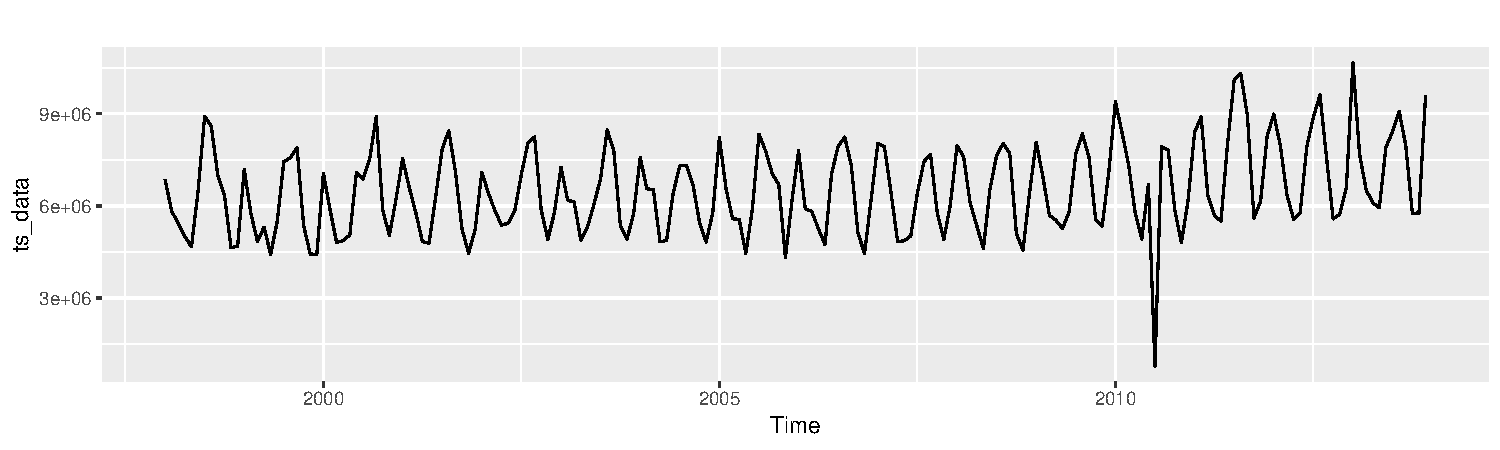
\includegraphics{Part-B-AS_files/figure-latex/unnamed-chunk-3-1.pdf}

\begin{Shaded}
\begin{Highlighting}[]
\CommentTok{# seasonal plot}
\KeywordTok{ggseasonplot}\NormalTok{(ts_data)}
\end{Highlighting}
\end{Shaded}

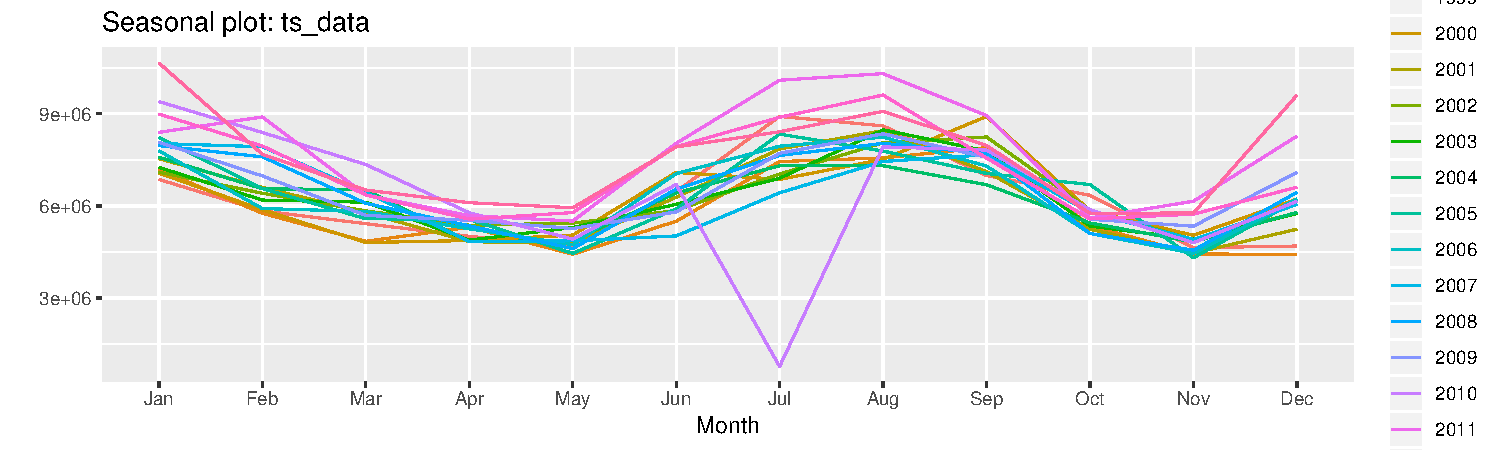
\includegraphics{Part-B-AS_files/figure-latex/unnamed-chunk-3-2.pdf}

\begin{Shaded}
\begin{Highlighting}[]
\CommentTok{# sub-seasonal plot}
\KeywordTok{ggsubseriesplot}\NormalTok{(ts_data)}
\end{Highlighting}
\end{Shaded}

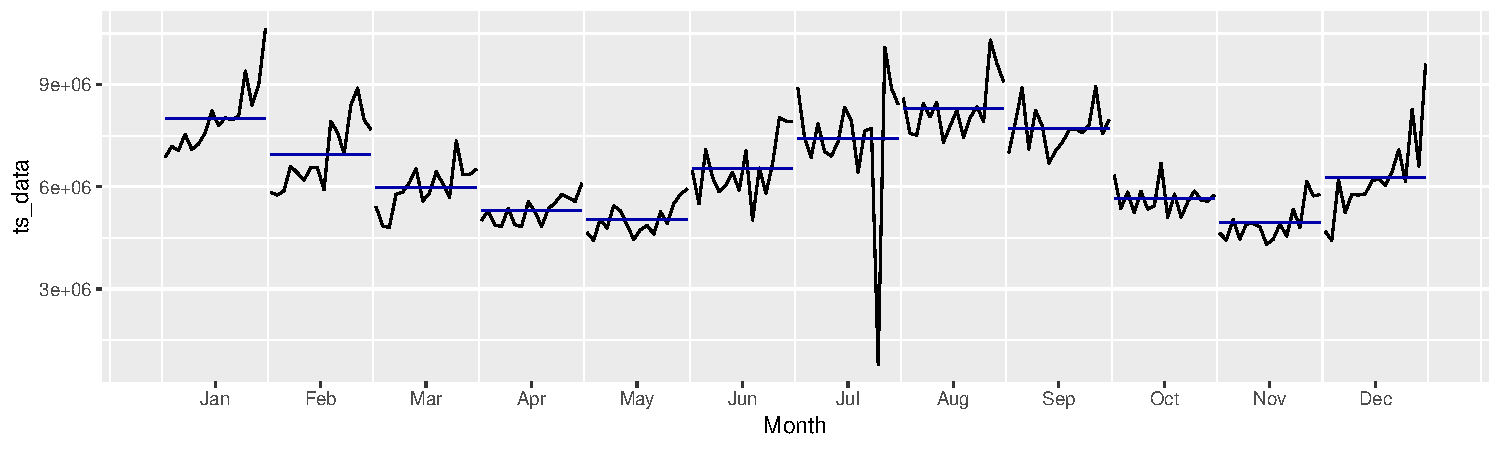
\includegraphics{Part-B-AS_files/figure-latex/unnamed-chunk-3-3.pdf}

\begin{Shaded}
\begin{Highlighting}[]
\CommentTok{# STL decomposition}
\KeywordTok{stl}\NormalTok{(ts_data, }\DataTypeTok{s.window =} \StringTok{'periodic'}\NormalTok{) }\OperatorTok\StringTok{ }\KeywordTok{autoplot}\NormalTok{()}
\end{Highlighting}
\end{Shaded}

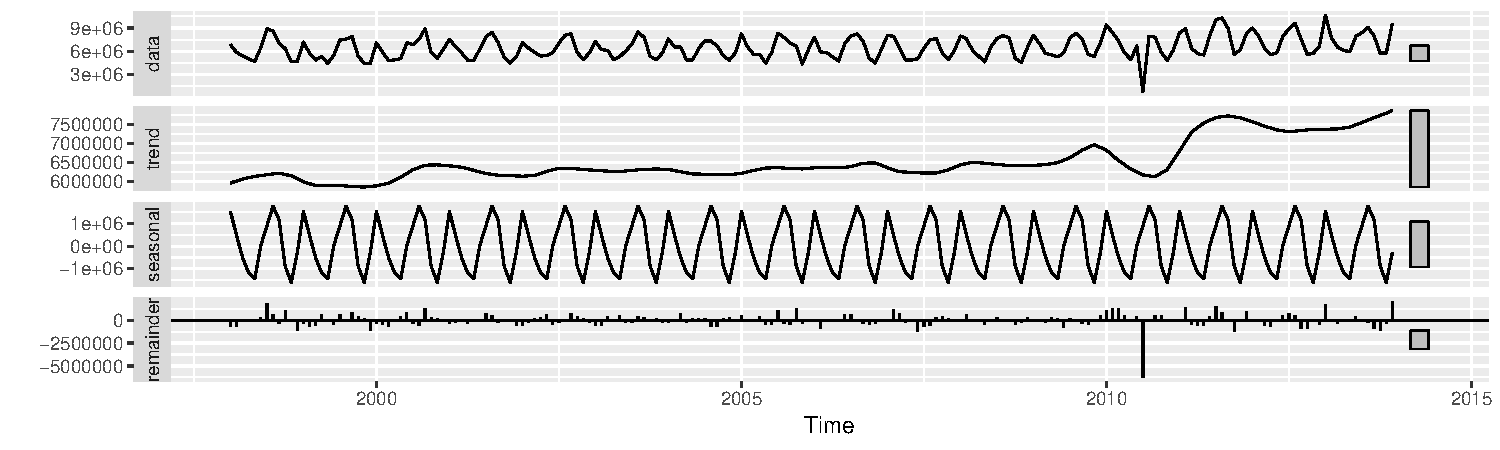
\includegraphics{Part-B-AS_files/figure-latex/unnamed-chunk-3-4.pdf}

\begin{Shaded}
\begin{Highlighting}[]
\CommentTok{# Autocorrelation}
\KeywordTok{ggAcf}\NormalTok{(ts_data)}
\end{Highlighting}
\end{Shaded}

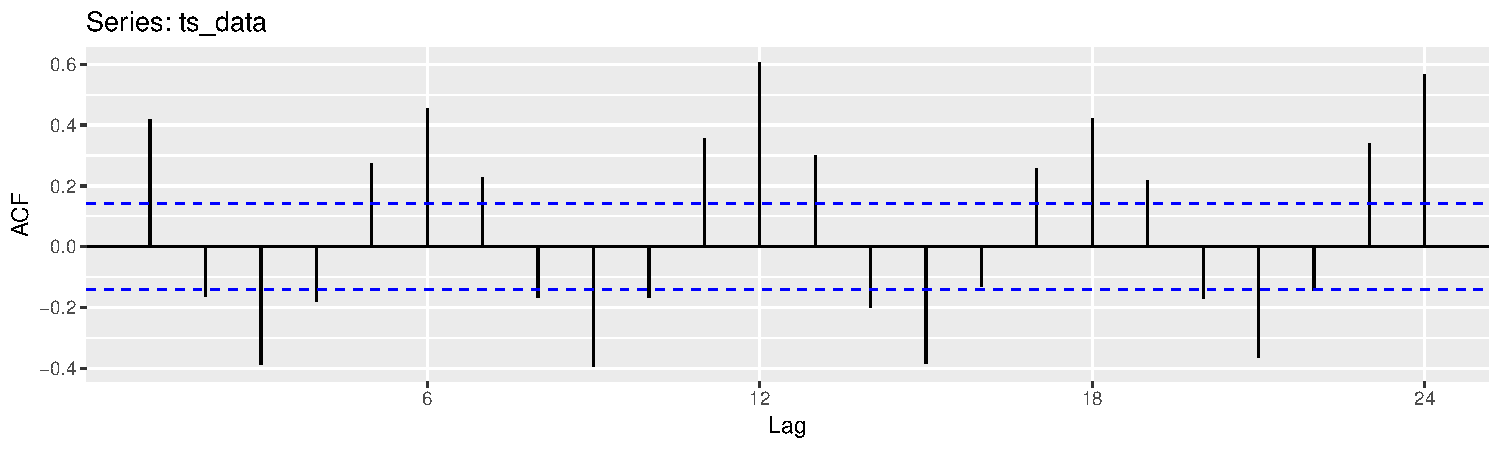
\includegraphics{Part-B-AS_files/figure-latex/unnamed-chunk-3-5.pdf}

\begin{Shaded}
\begin{Highlighting}[]
\KeywordTok{Box.test}\NormalTok{(ts_data, }\DataTypeTok{type =} \KeywordTok{c}\NormalTok{(}\StringTok{"Ljung-Box"}\NormalTok{))}
\end{Highlighting}
\end{Shaded}

\begin{verbatim}
FALSE 
FALSE   Box-Ljung test
FALSE 
FALSE data:  ts_data
FALSE X-squared = 34.118, df = 1, p-value = 5.187e-09
\end{verbatim}

\begin{Shaded}
\begin{Highlighting}[]
\CommentTok{# summary statistics}
\KeywordTok{summary}\NormalTok{(ts_data)}
\end{Highlighting}
\end{Shaded}

\begin{verbatim}
FALSE     Min.  1st Qu.   Median     Mean  3rd Qu.     Max. 
FALSE   770523  5434539  6314472  6508724  7649733 10655730
\end{verbatim}

\begin{Shaded}
\begin{Highlighting}[]
\KeywordTok{summary}\NormalTok{(power_data)}
\end{Highlighting}
\end{Shaded}

\begin{verbatim}
FALSE   CaseSequence     YYYY-MMM              KWH          
FALSE  Min.   :733.0   Length:192         Min.   :  770523  
FALSE  1st Qu.:780.8   Class :character   1st Qu.: 5434539  
FALSE  Median :828.5   Mode  :character   Median : 6314472  
FALSE  Mean   :828.5                      Mean   : 6508724  
FALSE  3rd Qu.:876.2                      3rd Qu.: 7649733  
FALSE  Max.   :924.0                      Max.   :10655730
\end{verbatim}

\begin{Shaded}
\begin{Highlighting}[]
\CommentTok{# Boxplot}
\KeywordTok{boxplot}\NormalTok{(ts_data}\OperatorTok{~}\KeywordTok{cycle}\NormalTok{(ts_data))}
\end{Highlighting}
\end{Shaded}

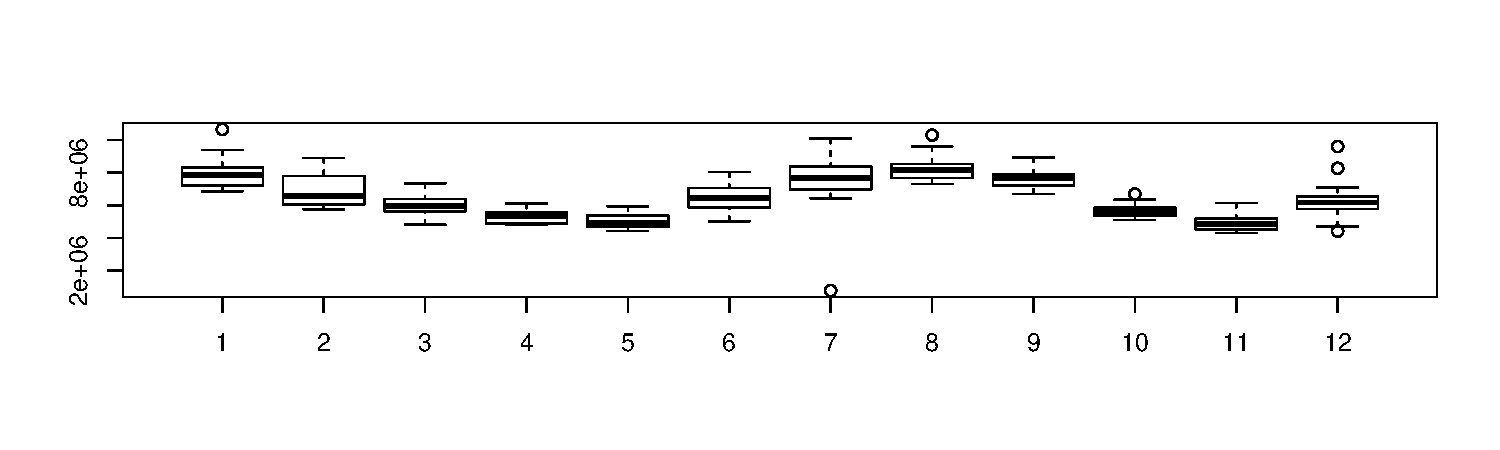
\includegraphics{Part-B-AS_files/figure-latex/unnamed-chunk-3-6.pdf}

\hypertarget{data-model}{%
\section{Data Model}\label{data-model}}

From residual test (Box-Ljung), we found that ets - MNM is not reliable
predictor as residuals are not white noise. Other models are all valid
as residuals are all white noise (p \textgreater{} 0.05 from
checkresiduals()). We will compare Arima and ets - AAN and ets - AAdN
from stl decomposition in terms of RMSE on test set in the next section.

\hypertarget{model-1-arima}{%
\subsection{Model \#1: ARIMA}\label{model-1-arima}}

\begin{Shaded}
\begin{Highlighting}[]
\CommentTok{# auto.arima}
\NormalTok{arima_model <-}\StringTok{ }\KeywordTok{auto.arima}\NormalTok{(ts_data)}

\CommentTok{# forecast values}
\NormalTok{arima_model <-}\StringTok{ }\KeywordTok{forecast}\NormalTok{(arima_model, }\DataTypeTok{h=}\DecValTok{3}\NormalTok{)}

\CommentTok{# forecast plot}
\KeywordTok{autoplot}\NormalTok{(arima_model) }\OperatorTok{+}\StringTok{ }\KeywordTok{autolayer}\NormalTok{(}\KeywordTok{fitted}\NormalTok{(arima_model))}
\end{Highlighting}
\end{Shaded}

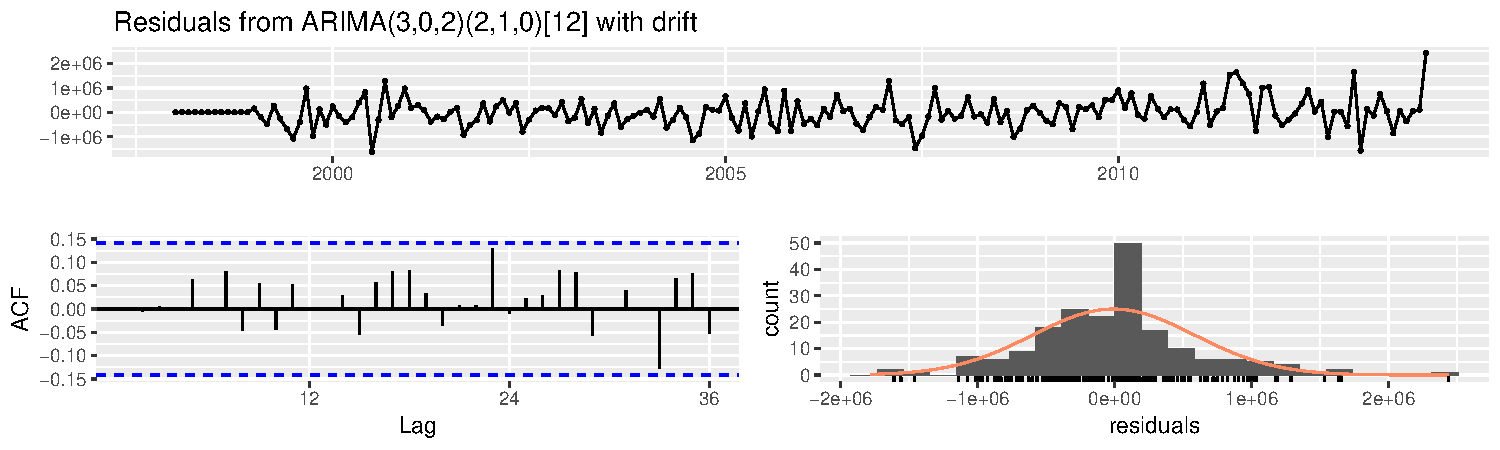
\includegraphics{Part-B-AS_files/figure-latex/unnamed-chunk-4-1.pdf}

\begin{Shaded}
\begin{Highlighting}[]
\KeywordTok{accuracy}\NormalTok{(arima_model)}
\end{Highlighting}
\end{Shaded}

\begin{verbatim}
FALSE                     ME     RMSE      MAE       MPE     MAPE      MASE
FALSE Training set -25755.56 823918.8 489803.5 -5.518168 11.63252 0.7141674
FALSE                   ACF1
FALSE Training set 0.0130951
\end{verbatim}

\begin{Shaded}
\begin{Highlighting}[]
\KeywordTok{checkresiduals}\NormalTok{(arima_model)}
\end{Highlighting}
\end{Shaded}

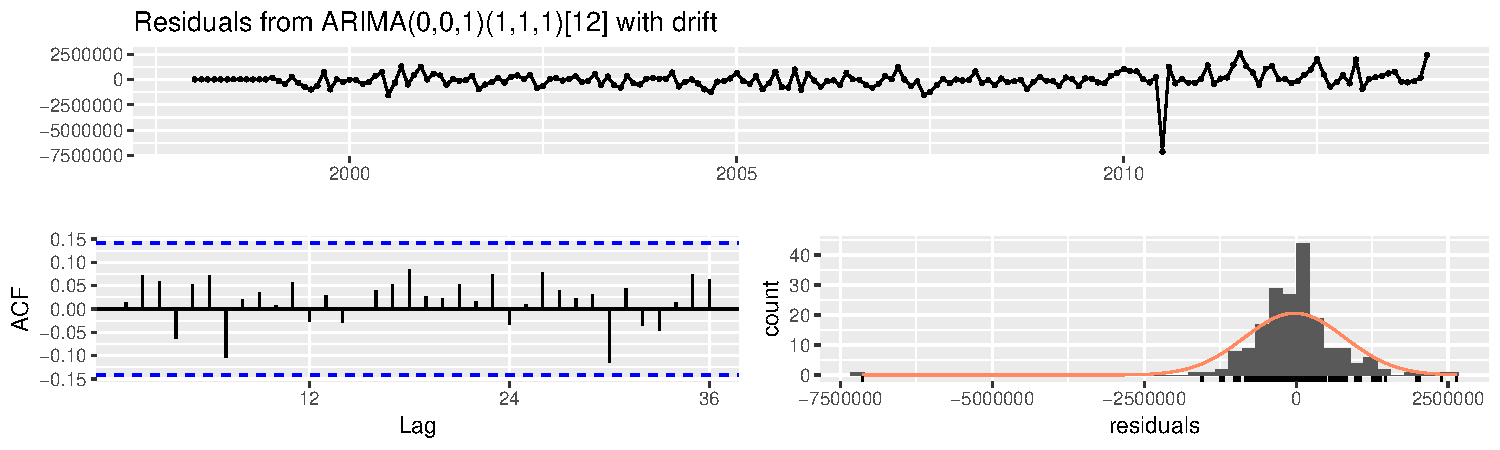
\includegraphics{Part-B-AS_files/figure-latex/unnamed-chunk-4-2.pdf}

\begin{verbatim}
FALSE 
FALSE   Ljung-Box test
FALSE 
FALSE data:  Residuals from ARIMA(0,0,1)(1,1,1)[12] with drift
FALSE Q* = 12.619, df = 20, p-value = 0.8931
FALSE 
FALSE Model df: 4.   Total lags used: 24
\end{verbatim}

\hypertarget{model-2-stl-no-demped---ann}{%
\subsection{Model \#2: STL (no-demped) -
ANN}\label{model-2-stl-no-demped---ann}}

\begin{Shaded}
\begin{Highlighting}[]
\CommentTok{#stlf - etsmodel estimation --- A,N,N is chosen.}
\NormalTok{stl_ndemp <-}\StringTok{ }\KeywordTok{stlf}\NormalTok{(ts_data, }\DataTypeTok{damped=}\OtherTok{FALSE}\NormalTok{, }\DataTypeTok{s.window =} \StringTok{"periodic"}\NormalTok{, }\DataTypeTok{robust=}\OtherTok{TRUE}\NormalTok{, }\DataTypeTok{h =} \DecValTok{3}\NormalTok{)}

\CommentTok{# forecast plot}
\KeywordTok{autoplot}\NormalTok{(stl_ndemp) }\OperatorTok{+}\StringTok{ }\KeywordTok{autolayer}\NormalTok{(}\KeywordTok{fitted}\NormalTok{(stl_ndemp))}
\end{Highlighting}
\end{Shaded}

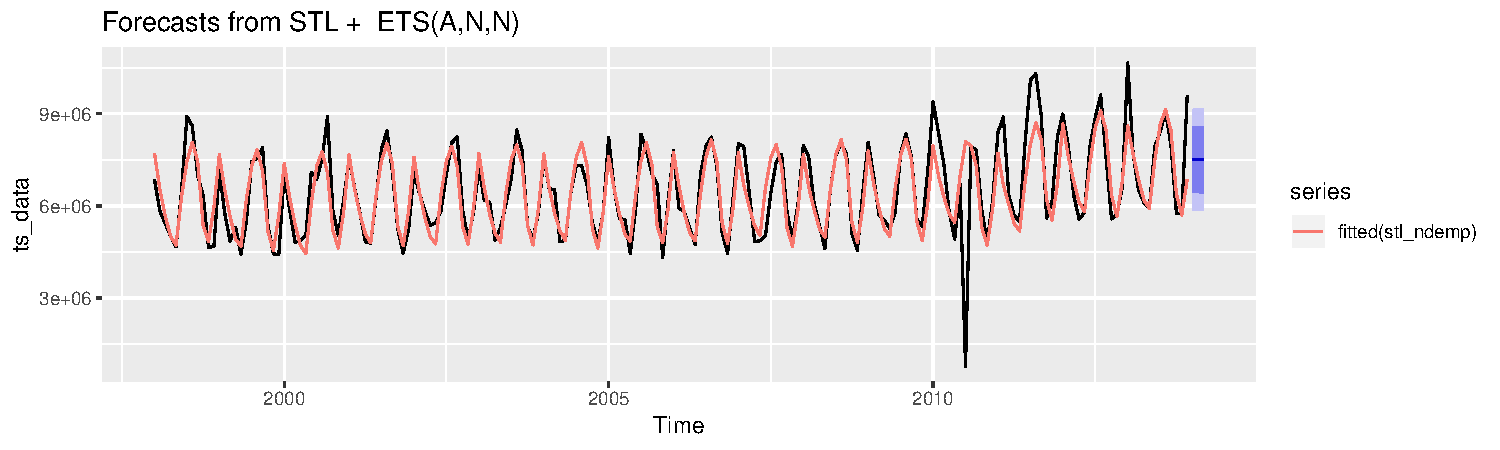
\includegraphics{Part-B-AS_files/figure-latex/unnamed-chunk-5-1.pdf}

\begin{Shaded}
\begin{Highlighting}[]
\KeywordTok{checkresiduals}\NormalTok{(stl_ndemp)}
\end{Highlighting}
\end{Shaded}

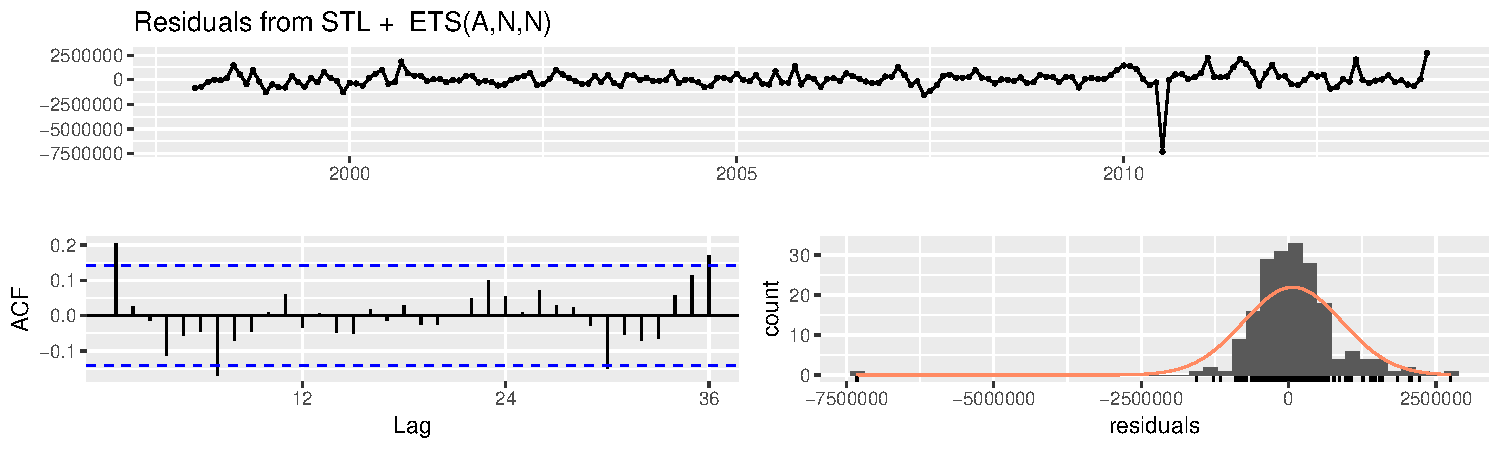
\includegraphics{Part-B-AS_files/figure-latex/unnamed-chunk-5-2.pdf}

\begin{verbatim}
FALSE 
FALSE   Ljung-Box test
FALSE 
FALSE data:  Residuals from STL +  ETS(A,N,N)
FALSE Q* = 25.094, df = 22, p-value = 0.2926
FALSE 
FALSE Model df: 2.   Total lags used: 24
\end{verbatim}

\hypertarget{model-2-2-stl-demped---aadn}{%
\subsection{Model \#2-2: STL (demped) -
AAdN}\label{model-2-2-stl-demped---aadn}}

\begin{Shaded}
\begin{Highlighting}[]
\CommentTok{#stlf - etsmodel estimation --- M, Ad, N is chosen.}
\NormalTok{stl_demp <-}\StringTok{ }\KeywordTok{stlf}\NormalTok{(ts_data, }\DataTypeTok{damped=}\OtherTok{TRUE}\NormalTok{, }\DataTypeTok{s.window =} \StringTok{"periodic"}\NormalTok{, }\DataTypeTok{robust=}\OtherTok{TRUE}\NormalTok{, }\DataTypeTok{h =} \DecValTok{3}\NormalTok{)}

\CommentTok{# forecast plot}
\KeywordTok{autoplot}\NormalTok{(stl_demp) }\OperatorTok{+}\StringTok{ }\KeywordTok{autolayer}\NormalTok{(}\KeywordTok{fitted}\NormalTok{(stl_demp))}
\end{Highlighting}
\end{Shaded}

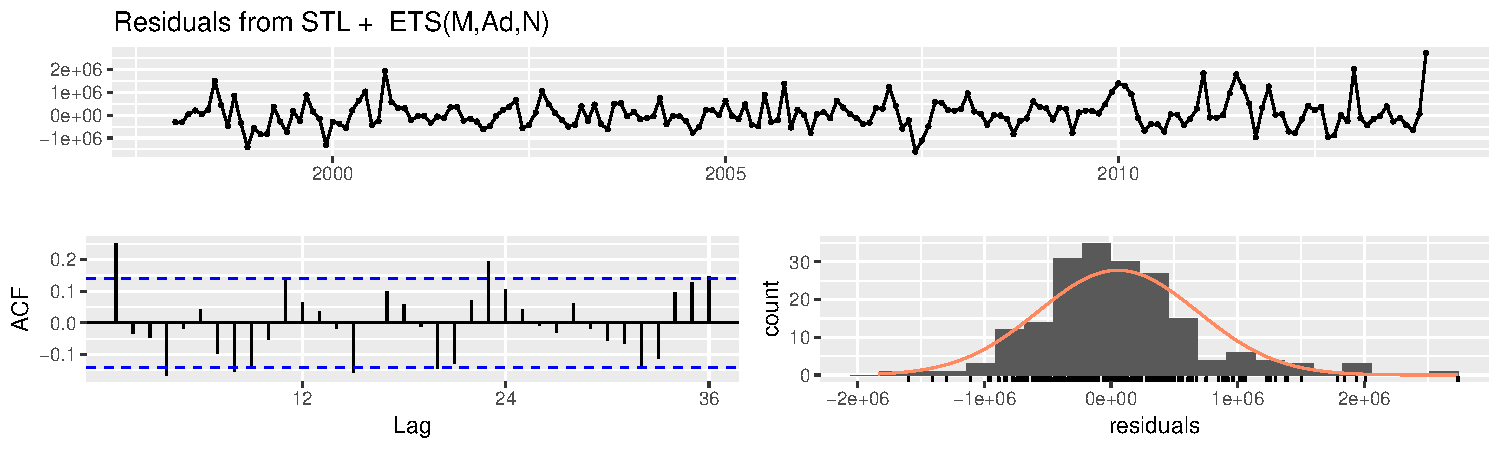
\includegraphics{Part-B-AS_files/figure-latex/unnamed-chunk-6-1.pdf}

\begin{Shaded}
\begin{Highlighting}[]
\KeywordTok{checkresiduals}\NormalTok{(stl_demp)}
\end{Highlighting}
\end{Shaded}

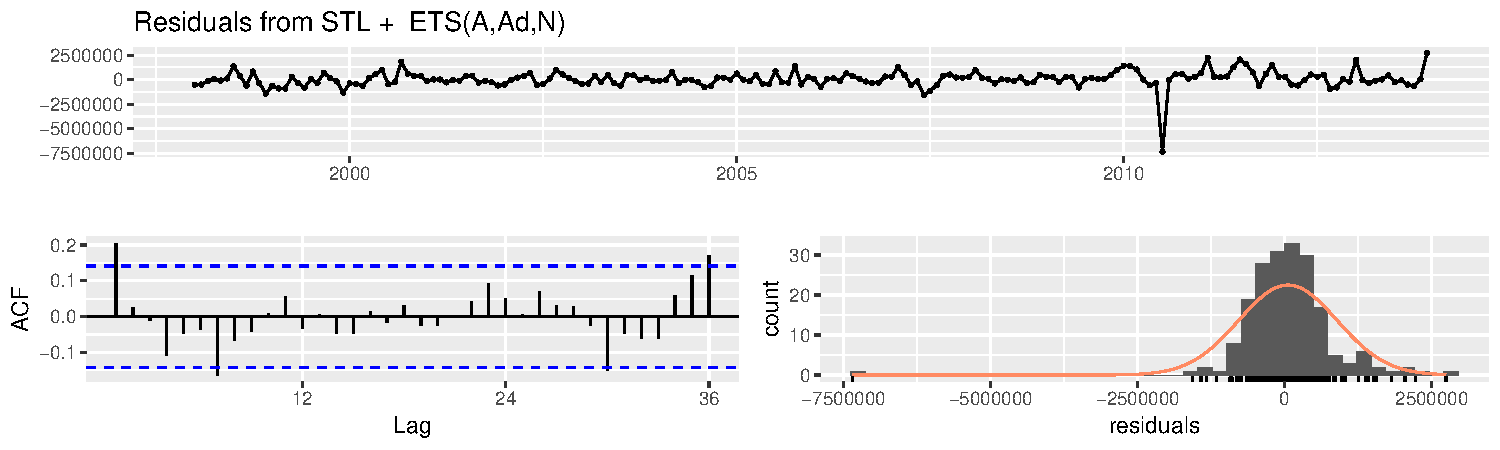
\includegraphics{Part-B-AS_files/figure-latex/unnamed-chunk-6-2.pdf}

\begin{verbatim}
FALSE 
FALSE   Ljung-Box test
FALSE 
FALSE data:  Residuals from STL +  ETS(A,Ad,N)
FALSE Q* = 23.407, df = 19, p-value = 0.2199
FALSE 
FALSE Model df: 5.   Total lags used: 24
\end{verbatim}

\hypertarget{model-3-ets---mnm}{%
\subsection{Model \#3: ets - MNM}\label{model-3-ets---mnm}}

\begin{Shaded}
\begin{Highlighting}[]
\CommentTok{# ETS models - MNM}
\NormalTok{ets_model <-}\StringTok{ }\KeywordTok{ets}\NormalTok{(ts_data)}

\CommentTok{# forecast plot}
\KeywordTok{autoplot}\NormalTok{(}\KeywordTok{forecast}\NormalTok{(ets_model, }\DataTypeTok{h=}\DecValTok{3}\NormalTok{)) }\OperatorTok{+}\StringTok{ }\KeywordTok{autolayer}\NormalTok{(}\KeywordTok{fitted}\NormalTok{(ets_model))}
\end{Highlighting}
\end{Shaded}

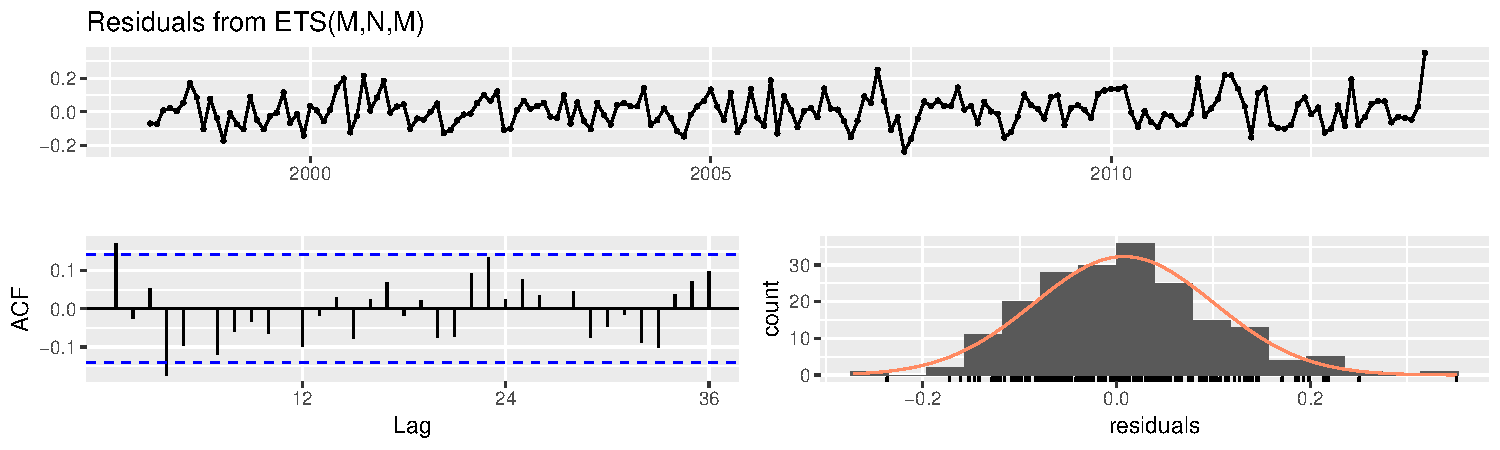
\includegraphics{Part-B-AS_files/figure-latex/unnamed-chunk-7-1.pdf}

\begin{Shaded}
\begin{Highlighting}[]
\KeywordTok{checkresiduals}\NormalTok{(ets_model)}
\end{Highlighting}
\end{Shaded}

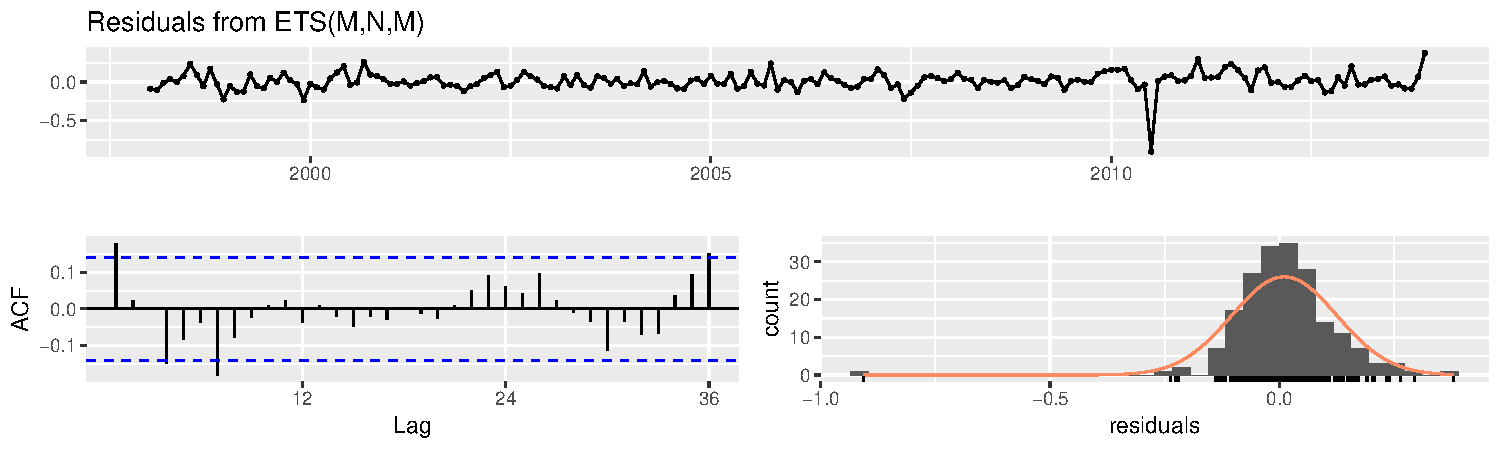
\includegraphics{Part-B-AS_files/figure-latex/unnamed-chunk-7-2.pdf}

\begin{verbatim}
FALSE 
FALSE   Ljung-Box test
FALSE 
FALSE data:  Residuals from ETS(M,N,M)
FALSE Q* = 25.272, df = 10, p-value = 0.004853
FALSE 
FALSE Model df: 14.   Total lags used: 24
\end{verbatim}

\hypertarget{forecast-accuracy}{%
\section{Forecast accuracy}\label{forecast-accuracy}}

Using Time series cross-validation, we compute RMSE on testset (h=3). We
will pick the model with the lowest RMSE on testset as our final model.

\hypertarget{model-1-arima-1}{%
\subsection{Model \#1: ARIMA}\label{model-1-arima-1}}

\begin{Shaded}
\begin{Highlighting}[]
\NormalTok{arima_cv <-}\StringTok{ }\ControlFlowTok{function}\NormalTok{(x, h)\{}\KeywordTok{forecast}\NormalTok{(}\KeywordTok{Arima}\NormalTok{(ts_data, }\DataTypeTok{order =} \KeywordTok{c}\NormalTok{(}\DecValTok{0}\NormalTok{, }\DecValTok{0}\NormalTok{, }\DecValTok{1}\NormalTok{), }\DataTypeTok{seasonal =} \KeywordTok{c}\NormalTok{(}\DecValTok{1}\NormalTok{, }\DecValTok{1}\NormalTok{, }\DecValTok{1}\NormalTok{),  }\DataTypeTok{include.drift =} \OtherTok{TRUE}\NormalTok{), }\DataTypeTok{h=}\NormalTok{h)\}}
\NormalTok{e <-}\StringTok{ }\KeywordTok{tsCV}\NormalTok{(ts_data, arima_cv, }\DataTypeTok{h=}\DecValTok{3}\NormalTok{)}

\KeywordTok{sqrt}\NormalTok{(}\KeywordTok{mean}\NormalTok{(e}\OperatorTok{^}\DecValTok{2}\NormalTok{, }\DataTypeTok{na.rm=}\OtherTok{TRUE}\NormalTok{))}
\end{Highlighting}
\end{Shaded}

\begin{verbatim}
FALSE [1] 2536394
\end{verbatim}

\hypertarget{model-2-stl-no-demped---ann-1}{%
\subsection{Model \#2: STL (no-demped) -
ANN}\label{model-2-stl-no-demped---ann-1}}

\begin{Shaded}
\begin{Highlighting}[]
\NormalTok{e <-}\StringTok{ }\KeywordTok{tsCV}\NormalTok{(ts_data, stlf, }\DataTypeTok{damped=}\OtherTok{FALSE}\NormalTok{, }\DataTypeTok{s.window =} \StringTok{"periodic"}\NormalTok{, }\DataTypeTok{robust=}\OtherTok{TRUE}\NormalTok{, }\DataTypeTok{h=}\DecValTok{3}\NormalTok{)}

\KeywordTok{sqrt}\NormalTok{(}\KeywordTok{mean}\NormalTok{(e}\OperatorTok{^}\DecValTok{2}\NormalTok{, }\DataTypeTok{na.rm=}\OtherTok{TRUE}\NormalTok{))}
\end{Highlighting}
\end{Shaded}

\begin{verbatim}
FALSE [1] 1467209
\end{verbatim}

\hypertarget{model-2-2-stl-demped---aadn-1}{%
\subsection{Model \#2-2: STL (demped) -
AAdN}\label{model-2-2-stl-demped---aadn-1}}

\begin{Shaded}
\begin{Highlighting}[]
\NormalTok{e <-}\StringTok{ }\KeywordTok{tsCV}\NormalTok{(ts_data, stlf, }\DataTypeTok{damped=}\OtherTok{TRUE}\NormalTok{, }\DataTypeTok{s.window =} \StringTok{"periodic"}\NormalTok{, }\DataTypeTok{robust=}\OtherTok{TRUE}\NormalTok{, }\DataTypeTok{h=}\DecValTok{3}\NormalTok{)}

\KeywordTok{sqrt}\NormalTok{(}\KeywordTok{mean}\NormalTok{(e}\OperatorTok{^}\DecValTok{2}\NormalTok{, }\DataTypeTok{na.rm=}\OtherTok{TRUE}\NormalTok{))}
\end{Highlighting}
\end{Shaded}

\begin{verbatim}
FALSE [1] 1473538
\end{verbatim}

\hypertarget{discussion}{%
\section{Discussion}\label{discussion}}

From above, we found that ARIMA is the worst predictor and STL (demped)
- AAdN is the best model as RMSE on testset is the lowest. We will pick
Model \#2-2.


\end{document}
